
\chapter{实验过程与分析}

\section{实验环境}
对于前面提出的基于图像的树木轻量化建模方法,本文做了大量实验验证了其可行性。
本文使用的拍摄工具是高分辨率安卓手机索尼LT26ii,该手机最高分辨率能达到4000x3000,
已经足够实验的需求。拍摄地点为同济大学嘉定校区以及某住宅小区。本文实验所使用计算机
操作系统平台为XUbuntu 12.04,CPU为双核Intel(R) Core(TM) i5-3230M @ 2.60GHz。显卡为
NVidia GeForce GT750M。 所有实验程序均使用C/C++语言完成,使用g++编译器进行编译,
同时使用OpenGL version 4.3图形硬件接口来完成可视化工作。

\section{实验结果与分析}
本文以三棵树的建模结果作为展示和分析的依据,其中第一棵树拍摄帧数为20帧,见图\ref{fig:sample1}。
第二棵树的拍摄帧数为12帧,见图\ref{fig:sample2}。第三棵树的拍摄帧数为20帧,见图\ref{fig:sample3}。

% sample 1
\begin{figure}[H]
	\captionsetup[subfigure]{labelformat=empty}
	\subfloat[]{
	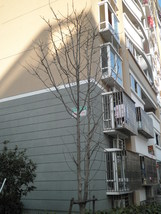
\includegraphics[height=2cm]{sample1_1.jpg}}
	\hspace{1mm}
	\subfloat[]{
	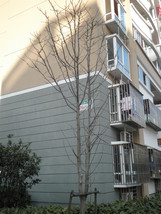
\includegraphics[height=2cm]{sample1_2.jpg}}
	\hspace{1mm}
	\subfloat[]{
	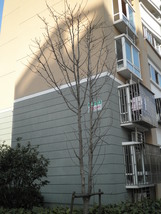
\includegraphics[height=2cm]{sample1_3.jpg}}
	\hspace{1mm}
	\subfloat[]{
	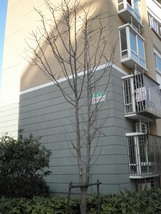
\includegraphics[height=2cm]{sample1_4.jpg}}
	\hspace{1mm}
	\subfloat[]{
	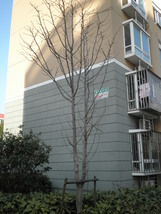
\includegraphics[height=2cm]{sample1_5.jpg}}
	\hspace{1mm}
	\subfloat[]{
	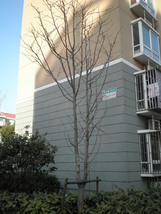
\includegraphics[height=2cm]{sample1_6.jpg}}
	\hspace{1mm}
	\subfloat[]{
	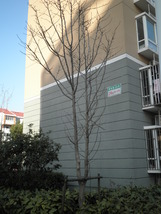
\includegraphics[height=2cm]{sample1_7.jpg}}
	\hspace{1mm}
	\subfloat[]{
	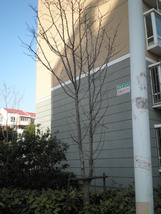
\includegraphics[height=2cm]{sample1_8.jpg}}
	\hspace{1mm}
	\subfloat[]{
	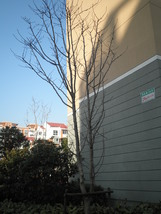
\includegraphics[height=2cm]{sample1_9.jpg}}
	\hspace{1mm}
	\subfloat[]{
	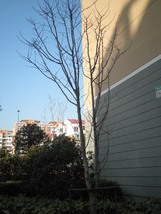
\includegraphics[height=2cm]{sample1_10.jpg}}
	\hspace{1mm}
	\subfloat[]{
	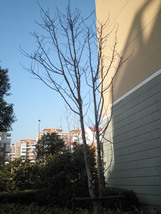
\includegraphics[height=2cm]{sample1_11.jpg}}
	\hspace{1mm}
	\subfloat[]{
	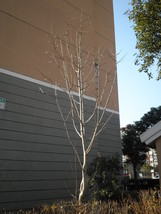
\includegraphics[height=2cm]{sample1_12.jpg}}
	\hspace{1mm}
	\subfloat[]{
	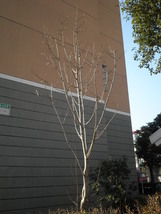
\includegraphics[height=2cm]{sample1_13.jpg}}
	\hspace{1mm}
	\subfloat[]{
	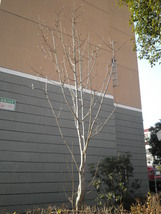
\includegraphics[height=2cm]{sample1_14.jpg}}
	\hspace{1mm}
	\subfloat[]{
	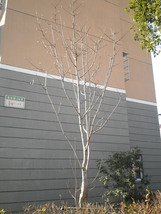
\includegraphics[height=2cm]{sample1_15.jpg}}
	\hspace{1mm}
	\subfloat[]{
	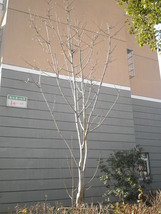
\includegraphics[height=2cm]{sample1_16.jpg}}
	\hspace{1mm}
	\subfloat[]{
	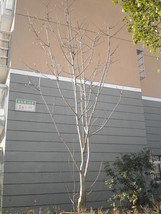
\includegraphics[height=2cm]{sample1_17.jpg}}
	\hspace{1mm}
	\subfloat[]{
	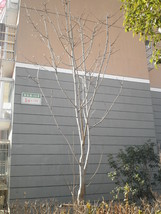
\includegraphics[height=2cm]{sample1_18.jpg}}
	\hspace{1mm}
	\subfloat[]{
	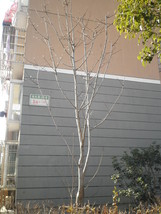
\includegraphics[height=2cm]{sample1_19.jpg}}
	\hspace{1mm}
	\subfloat[]{
	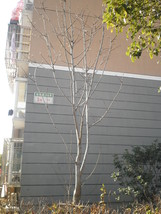
\includegraphics[height=2cm]{sample1_20.jpg}}
	\hspace{1mm}
	\caption{树木1图像序列,帧数为20帧,拍摄地点为某住宅小区}
	\label{fig:sample1}
\end{figure}

% sample 2
\begin{figure}[H]
	\captionsetup[subfigure]{labelformat=empty}
	\subfloat[]{
	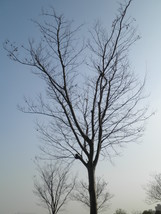
\includegraphics[height=2cm]{sample2_1.jpg}}
	\hspace{1mm}
	\subfloat[]{
	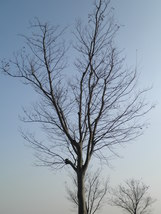
\includegraphics[height=2cm]{sample2_2.jpg}}
	\hspace{1mm}
	\subfloat[]{
	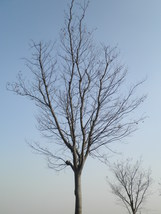
\includegraphics[height=2cm]{sample2_3.jpg}}
	\hspace{1mm}
	\subfloat[]{
	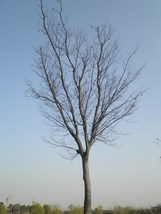
\includegraphics[height=2cm]{sample2_4.jpg}}
	\hspace{1mm}
	\subfloat[]{
	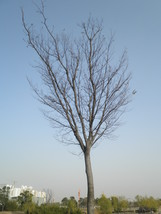
\includegraphics[height=2cm]{sample2_5.jpg}}
	\hspace{1mm}
	\subfloat[]{
	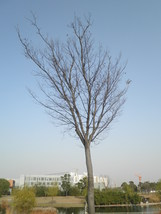
\includegraphics[height=2cm]{sample2_6.jpg}}
	\hspace{1mm}
	\subfloat[]{
	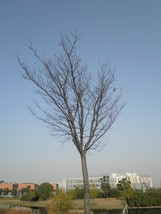
\includegraphics[height=2cm]{sample2_7.jpg}}
	\hspace{1mm}
	\subfloat[]{
	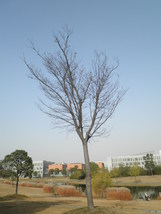
\includegraphics[height=2cm]{sample2_8.jpg}}
	\hspace{1mm}
	\subfloat[]{
	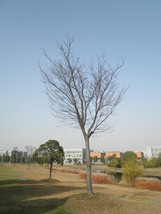
\includegraphics[height=2cm]{sample2_9.jpg}}
	\hspace{1mm}
	\subfloat[]{
	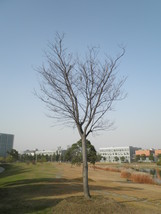
\includegraphics[height=2cm]{sample2_10.jpg}}
	\hspace{1mm}
	\subfloat[]{
	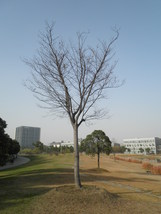
\includegraphics[height=2cm]{sample2_11.jpg}}
	\hspace{1mm}
	\subfloat[]{
	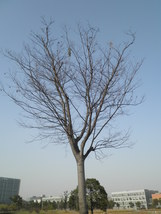
\includegraphics[height=2cm]{sample2_12.jpg}}
	\caption{树木2图像序列,帧数为12帧,拍摄地点为同济大学嘉定校区}
	\label{fig:sample2}
\end{figure}


% sample 3
\begin{figure}[H]
	\captionsetup[subfigure]{labelformat=empty}
	\subfloat[]{
	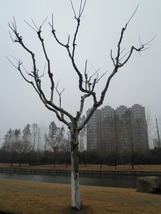
\includegraphics[height=2cm]{sample3_1.jpg}}
	\hspace{1mm}
	\subfloat[]{
	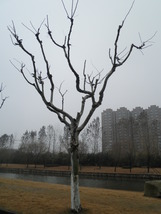
\includegraphics[height=2cm]{sample3_2.jpg}}
	\hspace{1mm}
	\subfloat[]{
	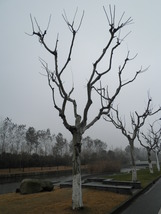
\includegraphics[height=2cm]{sample3_3.jpg}}
	\hspace{1mm}
	\subfloat[]{
	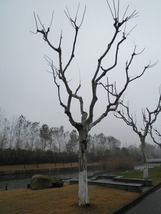
\includegraphics[height=2cm]{sample3_4.jpg}}
	\hspace{1mm}
	\subfloat[]{
	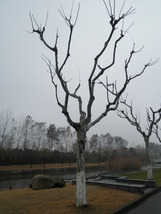
\includegraphics[height=2cm]{sample3_5.jpg}}
	\hspace{1mm}
	\subfloat[]{
	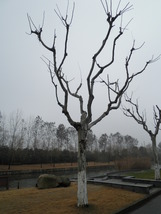
\includegraphics[height=2cm]{sample3_6.jpg}}
	\hspace{1mm}
	\subfloat[]{
	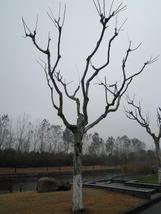
\includegraphics[height=2cm]{sample3_7.jpg}}
	\hspace{1mm}
	\subfloat[]{
	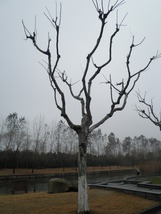
\includegraphics[height=2cm]{sample3_8.jpg}}
	\hspace{1mm}
	\subfloat[]{
	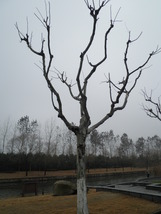
\includegraphics[height=2cm]{sample3_9.jpg}}
	\hspace{1mm}
	\subfloat[]{
	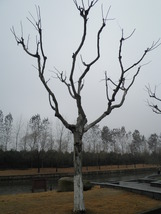
\includegraphics[height=2cm]{sample3_10.jpg}}
	\hspace{1mm}
	\subfloat[]{
	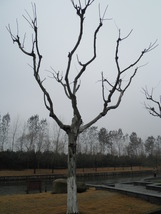
\includegraphics[height=2cm]{sample3_11.jpg}}
	\hspace{1mm}
	\subfloat[]{
	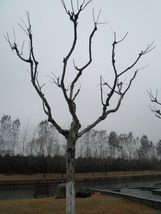
\includegraphics[height=2cm]{sample3_12.jpg}}
	\hspace{1mm}
	\subfloat[]{
	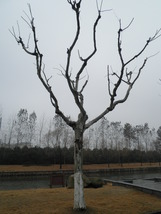
\includegraphics[height=2cm]{sample3_13.jpg}}
	\hspace{1mm}
	\subfloat[]{
	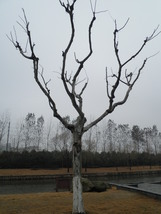
\includegraphics[height=2cm]{sample3_14.jpg}}
	\hspace{1mm}
	\subfloat[]{
	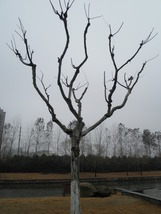
\includegraphics[height=2cm]{sample3_15.jpg}}
	\hspace{1mm}
	\subfloat[]{
	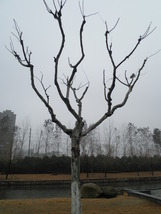
\includegraphics[height=2cm]{sample3_16.jpg}}
	\hspace{1mm}
	\subfloat[]{
	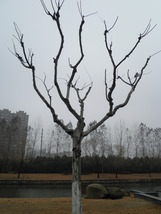
\includegraphics[height=2cm]{sample3_17.jpg}}
	\hspace{1mm}
	\subfloat[]{
	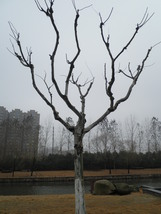
\includegraphics[height=2cm]{sample3_18.jpg}}
	\hspace{1mm}
	\subfloat[]{
	\includegraphics[height=2cm]{sample3_19.jpg}}
	\hspace{1mm}
	\subfloat[]{
	\includegraphics[height=2cm]{sample3_20.jpg}}
	\hspace{1mm}
	\caption{树木3图像序列,帧数为20帧,拍摄地点为同济大学嘉定校区}
	\label{fig:sample3}
\end{figure}

本文还给出了每个图片序列三维重建出的点云模型、从点云模型中直接抽取的骨架模型以及
经过枝干合并方法轻量化得到的骨架模型。为了从直观上比较重建模型和图片序列的相似度,
本文从正面和侧面对所得模型进行投影,以方便从二维的视角判断其相似程度。图\ref{fig:s1proj1}和
图\ref{fig:s1proj2}分别给出了树木样本1在正面投影和侧面投影的比对情况。图\ref{fig:s2proj1}和
图\ref{fig:s2proj2}分别给出了树木样本2在正面投影和侧面投影的比对情况。图\ref{fig:s3proj1}和
图\ref{fig:s3proj2}分别给出了树木样本3在正面投影和侧面投影的比对情况。
\begin{figure}[H]
	\centering
	\subfloat[树木正面图像]{\includegraphics[width=6cm]{s1img1.jpg}}\hspace{3em}
	\subfloat[树木点云模型]{\includegraphics[width=6cm]{s1point1.png}}\hspace{3em}
	\subfloat[树木骨架模型]{\includegraphics[width=6cm]{s1skl1.png}}\hspace{3em}
	\subfloat[树木轻量化骨架模型]{\includegraphics[width=6cm]{s1lw1.png}}\hspace{3em}
	\caption{树木样本1正面投影比对}
	\label{fig:s1proj1}
\end{figure}
\begin{figure}
	\centering
	\subfloat[树木侧面图像]{\includegraphics[width=4.5cm]{s1img2.jpg}}\hspace{3em}
	\subfloat[树木点云模型]{\includegraphics[width=4.5cm]{s1point2.png}}\hspace{3em}
	\subfloat[树木骨架模型]{\includegraphics[width=4.5cm]{s1skl2.png}}\hspace{3em}
	\subfloat[树木轻量化骨架模型]{\includegraphics[width=4.5cm]{s1lw2.png}}\hspace{3em}
	\caption{树木样本1侧面投影比对}
	\label{fig:s1proj2}
\end{figure}
\begin{figure}
	\centering
	\subfloat[树木正面图像]{\includegraphics[width=6cm]{s2img1.jpg}}\hspace{3em}
	\subfloat[树木点云模型]{\includegraphics[width=6cm]{s2point1.png}}\hspace{3em}
	\subfloat[树木骨架模型]{\includegraphics[width=6cm]{s2skl1.png}}\hspace{3em}
	\subfloat[树木轻量化骨架模型]{\includegraphics[width=6cm]{s2lw1.png}}\hspace{3em}
	\caption{树木样本2正面投影比对}
	\label{fig:s2proj1}
\end{figure}
\begin{figure}
	\centering
	\subfloat[树木侧面图像]{\includegraphics[width=6cm]{s2img2.jpg}}\hspace{3em}
	\subfloat[树木点云模型]{\includegraphics[width=6cm]{s2point2.png}}\hspace{3em}
	\subfloat[树木骨架模型]{\includegraphics[width=6cm]{s2skl2.png}}\hspace{3em}
	\subfloat[树木轻量化骨架模型]{\includegraphics[width=6cm]{s2lw2.png}}\hspace{3em}
	\caption{树木样本2侧面投影比对}
	\label{fig:s2proj2}
\end{figure}
\begin{figure}
	\centering
	\subfloat[树木正面图像]{\includegraphics[width=6cm]{s3img1.jpg}}\hspace{3em}
	\subfloat[树木点云模型]{\includegraphics[width=6cm]{s3point1.png}}\hspace{3em}
	\subfloat[树木骨架模型]{\includegraphics[width=6cm]{s3skl1.png}}\hspace{3em}
	\subfloat[树木轻量化骨架模型]{\includegraphics[width=6cm]{s3lw1.png}}\hspace{3em}
	\caption{树木样本3正面投影比对}
	\label{fig:s3proj1}
\end{figure}
\begin{figure}
	\centering
	\subfloat[树木侧面图像]{\includegraphics[width=6cm]{s3img2.jpg}}\hspace{3em}
	\subfloat[树木点云模型]{\includegraphics[width=6cm]{s3point2.png}}\hspace{3em}
	\subfloat[树木骨架模型]{\includegraphics[width=6cm]{s3skl2.png}}\hspace{3em}
	\subfloat[树木轻量化骨架模型]{\includegraphics[width=6cm]{s3lw2.png}}\hspace{3em}
	\caption{树木样本3侧面投影比对}
	\label{fig:s3proj2}
\end{figure}

可以看出,无论从正面还是侧面,通过本文轻量化建模方法所得到的树木模型都具有很高的还原
性。由于树木1和树木的细小枝干比较多,所以对于其细节部分的还原度还有待提升。但是类似
树木3这种不含太多细小枝干的树木,本文可以给出很高的还原度。从另一方面来看,由于本文
的方法是轻量化建模,对于细小的枝干的舍弃也是无法避免的,所以从总体来看本文的方法对于
真实树木的轻量化建模效果还是十分客观的。

表\ref{tab:restore}分别对图片序列信息量、三维重建还原度、骨架抽取还原度以及总的还原度给出了量化
的实验计算结果。注意,图片序列信息量的计算,本文根据实验所得的最佳$a/b=0.8$的结果来进行计算。
从表中可以看出,树木样本3的还原度最高,而树木样本2的还原度最低。分别比较它们的三维重建还原
度和骨架抽取还原度可以看出,图片数量的越多,样本结构越简单,则三维还原度的还原度就越高。
而对于树木结构复杂的树木,骨架抽取是一个难点,因为树木分支结构的复杂性容易引起骨架抽取的
二义性从而导致抽取不准确,所以对于样本3这样结构简单的树木来说,骨架抽取还原度最高,而对于
结构最复杂,细枝最多的样本2来说,骨架抽取还原度最低。
\\
\begin{table}[H]
	\caption{树木样本还原度统计}
	\centering
\begin{tabular}{c|cccc} \label{tab:restore}
	树木样本& 图片序列信息量 & 三维重建还原度 & 骨架抽取还原度 & 总还原度\\
	\hline
	1		& 0.988			 & 0.892		  & 0.871		   & 0.767\\
	2		& 0.931			 & 0.849		  & 0.852		   & 0.673\\
	3		& 0.988			 & 0.935		  & 0.953		   & 0.881\\
\end{tabular}
\end{table}

表\ref{tab:lw}从轻量化的角度,对比了三个树木样本从三维重建得到的点云数据文件的体积、
骨架抽取后得到的文件体积和经过轻量化以后得到的文件体积。从表中可以看出,三个样本从
点云数据到骨架数据体积都大大的减小了,对于以KB为单位的骨架体积,已经可以普及到一般的
Web应用来。对于后一步轻量化的步骤,主要是为了满足更高的应用需求,可以看出,对于骨架
结构中细枝较多的样本1和样本2,其轻量化所减小的模型体积比例要大于结构简单的样本3,这是
因为模型的轻量化主要是建立在对树木结构进行简化,而本来就比较简单的结构,这种轻量化的
程度就会减弱。
\\
\begin{table}[H]
	\caption{树木建模各阶段文件体积对比}
	\centering
	\begin{tabular}{c|ccc} \label{tab:lw}
		树木样本	&	三维重建点云体积	& 原骨架体积	& 轻量化骨架体积\\
		\hline
		1			&   2.5M				& 50.3K			& 8.2K\\
		2			&	4.4M				& 103.1K		& 15.1K\\
		3			&	2.2M				& 31.5K			& 7.3K\\
	\end{tabular}
\end{table}

\section{本章小节}
本章首先交代了本文所进行实验的软硬件平台等实验环境。然后给出了3个样本的实验结果,
从模型正面和侧面进行投影并从直观上比较了重建模型与输入图像序列的相似度。然后进一步运用
前一章给出的建模还原度的计算式,对三个样本进行了量化的计算,并分析了影响建模还原度
的一些因素。最后给出了3个样本重建模型的轻量化数据,并基于该分析了影响树木模型轻量化
的一些因素。从最后的实验结果,我们可以看出,本文提出的基于图像的轻量化建模方法具有
可行性和十分客观的重建效果。

